\documentclass[a4paper, 12pt]{amsart}
\usepackage[french]{babel}
\usepackage[utf8]{inputenc}
\usepackage{amssymb}
\usepackage{graphicx}
\usepackage{coursebook}
\fthmstyle{plain}
\newfancythm{fthm}{Théorème}
\fthmstyle{defn}
\newfancythm{fdefn}{Définition}
\fthmstyle{ex}
\newfancythm{fex}{Exercice}
%\DeclareMathOperator*{\ln}{ln}
\newcommand{\pd}[2]{\ensuremath{\frac{\partial #1}{\partial #2}}}

\title{Eléments de correction pour les exercices vus en cours}

\begin{document}
\maketitle
\section{Rappels}
Si $f$ est une application intégrable telle que:
\[
\int_\R \left | f(t) \right| dt < +\infty
\]
sa transformée de Fourier est l'application $\widehat{f}$ définie par:
\[
\widehat{f} \colon \omega \in \R \mapsto \int_{\R} f(t) \exp(-i \omega t ) dt
\]
\section{Fonctions de la variable complexe}
\begin{fex}
 Soit $\Omega$ un domaine non vide de $\mathbb{C}$ et soit $f$ application
holomorphe sur $\Omega$. Montrer que les conditions suivantes sont
équivalentes~:
\renewcommand{\theenumi}{\alph{enumi}}
\begin{enumerate}
\item $f$ est constante sur $\Omega$.
\item $\Re(f)$ est constante sur $\Omega$.
\item $\Im(f)$ est constante sur $\Omega$.
\item $|f|$ est constante sur $\Omega$.
\end{enumerate}
\end{fex}
On séparera partie réelle et partie imaginaire de $f$ en posant $f=P+iQ$
Il est clair que (a) implique les autres conditions. Si on suppose (b), par
application des conditions de Cauchy et en utilisant que $P$ est constant:
\[
 \pd{P}{x} = \pd{Q}{y} = 0 , \pd{P}{y}=-\pd{Q}{x} = 0
\]
$\Omega$ étant connexe, on en déduit $Q$ constante. Il s'agit en fait d'une
équivalence $(b) \Leftrightarrow (c)$, le même raisonnement s'appliquant à $Q$.
On montre donc en sus que $|f|^2=P^2+Q^2$ est aussi une constante.
Finalement, si l'on suppose $P^2+Q^2$ constant, les dérivées partielles de
cette application par rapport à $x,y$ donnent;
\[
 P\pd{P}{x}+Q\pd{Q}{x}= 0,\,  P\pd{P}{y}+Q\pd{Q}{y}= 0
\]
En utilisant les conditions de Cauchy:
\[
 P\pd{P}{x}-Q\pd{P}{y}= 0,\,  P\pd{P}{y}+Q\pd{P}{x}= 0
\]
Il s'agit d'un système linéaire homogène de déterminant $P^2+Q^2=|f|^2$. Si
cette quantité est nulle, alors $f$ est nulle et (a) est vérifiée. Sinon:
\[
 \pd{P}{x}=\pd{P}{y}=0
\]
prouvant que $P$ est une constante et donc aussi $Q$ car $(b) \Leftrightarrow
(c)$, soit $f$ constante.
\begin{fex}
 Soit la série entière:
\[
f \colon z \mapsto \sum_{n >0}(-1)^{n-1}\frac{(z-1)^n}{n}
\]
\begin{enumerate}
  \item Déterminer son rayon de convergence;
  \item Montrer que pour tout réel $x \in ]0,2[$, $f(x)=\log(x)$;
  \item En déduire que $f$ est l'unique application analytique prolongeant le
  logarithme réel sur le disque ouvert $B(1,1)$;
  \item Vérifier que sur $B(1,1)$, on a $\exp \circ f = Id$.
\end{enumerate}
\end{fex}
\begin{enumerate}
 \item On utilise le critère de d'Alembert. Le rapport de deux termes
consécutifs est $n/(n+1)$, de limite 1 à l'infini. Le rayon de convergence est
donc 1.
\item Résultat classique de classes préparatoires. On peut dériver terme à
terme la série dans son disque ouvert de convergence, qui donne la série:
\[
\sum_{n >0}(-1)^{n} (z-1)^n = \frac{1}{1+(z-1)}
\]
La valeur particulière $f(1)=0$ permet alors de conclure.
\item $f$ coïncide avec $\log$ sur une partie possèdant un point d'accumulation
(en fait, tout le segment réel $]0,2[$). Par le principe du prolongement
analytique, elle est unique.
\item Toujours sur le segment $]0,2[$, $\exp \circ f = \exp \circ \log = Id$.
Par prolongement analytique de l'application $\exp \circ f$, cette égalité est
vraie sur $B(1,1)$.
\end{enumerate}
\begin{fex}
Soit $\nu$ un entier. L'équation de Bessel d'ordre $\nu$ est:
\begin{equation}\label{eq:bessel}
z^2 \frac{d^2f}{dz^2} + z \frac{df}{dz} + \left(z^2-\nu^2\right)f = 0
\end{equation}
\begin{itemize}
\item Soit $f$ une solution de (\ref{eq:bessel}) que l'on suppose développable en série entière au voisinage de $0$. En écrivant son développement sous la forme:
\[
f \colon z \mapsto \sum_{n=0}^{+\infty} a_n x^{n+k}
\]
où $k$ est un entier, on a les relations:
\begin{eqnarray}
a_0 \left(k^2 - \nu^2\right) = 0 \\
a_1 \left(((k+1)^2 - \nu^2\right) = 0 \\
a_n \left((k+n)^2 - \nu^2\right) + a_{n-2} = 0, \, n \geq 2
\end{eqnarray}
\item En posant $k = \nu$, montrer que si $f$ solution de (\ref{eq:bessel}) est développable en série entière au voisinage de $0$ et vérifie $a_0=1/(2^\nu \nu!)$, son développement est:
\[
f \colon z \mapsto \left(\frac{z}{2}\right)^\nu \sum_{n=0}^{+\infty} \frac{(-1)^n}{n!(n+\nu)!}\left(\frac{z}{2}\right)^{2n}
\]
\item En utilisant le critère de Hadamard et la formule de Stirling:
\[
n! \sim_{+\infty} \sqrt{2 \pi n}\left(\frac{n}{e}\right)^n
\]
montrer que le rayon de convergence de la série est infini.
\end{itemize}
\end{fex}
\begin{enumerate}
\item Il s'agit d'une identification terme à terme des coefficients du développement de $f$.
\item Le choix particulier $k = \nu$ simplifie considérablement la récurrence
\[
a_n \left((k+n)^2 - \nu^2\right) + a_{n-2} = 0, \, n \geq 2
\]
qui devient:
\[
a_n \left(2\nu n + n^2\right) = - a_{n-2}, \, n \geq 2
\]
On en déduit~:
\[
a_n = a_0 \frac{(-1)^n\nu!}{2^{2n}n!(n+\nu)!}
\]
Le choix proposé de $a_0$ permet de retrouver les coefficients pairs proposés. Par ailleurs, on $a_1 =0$ et donc annulation de tous les coefficients impairs.
\item L'utilisation du critère de Hadamard est directe à partir de la formule de Stirling, le terme $a_n^{1/n}$ se comportant comme:
\[
\frac{1}{2\pi \sqrt{n(n+\nu)}\left(\frac{n}{e}\right)^{1+ \nu/2n}}
\]
au voisinage de $+\infty$. Il est à noter que le critère de d'Alembert nécessite une adaptation, car on ne peut former le rapport de deux termes consécutifs, tous les termes impairs étant nuls. 
\end{enumerate}
\begin{fex}
Soit $f$ une application de classe $C^k$ définie d'un ouvert $U$ de $\R^n$ dans $\R$. Montrer que l'expression:
\[
df = \sum_{i=1}^n \frac{\partial f}{\partial x_i} dx_i
\] 
définit une forme différentielle de degré $1$ dont on précisera la régularité.

\end{fex}
Il suffit de remarquer que $df$ est une combinaison linéaire des formes de base $dx_i, i=1\dots n$ avec des coefficients de classe $C^{k-1}$. On en déduit immédiatement qu'il s'agit d'une forme différentielle de degré $1$ et de régularité $C^{k-1}$.
\begin{fex}
En posant $\omega = \sum_{i=1}^n \omega_i dx_i$,
montrer que la forme $\phi^*\omega$ s'exprime sous la forme:
\[
\phi^*\omega = \sum_{j=1}^m \theta_j dx_j
\]
avec:
\[
\theta(x) = \phi^{\prime t} (x) \omega(\phi(x)) 
\]
où $\theta(x)$ (resp. $\omega(x)$) est le vecteur de composantes $\theta_j(x)$ (resp. $\omega_i(x)$) et $\phi^\prime(x)$ est la matrice de l'application dérivée de $\phi$ en $x$.
\end{fex}
On suppose que $\phi$ est définie sur un ouvert $V$ de $\R^m$ et prend ses valeurs dans un ouvert $U$ de $\R^n$. 
Par définition de l'image réciproque, on a pour tout point $y$ de $V$ et tout vecteur $v$ de $\R^m$:
\[
\phi^*\omega(y;v) = \omega(\phi(y);\phi^\prime(y).v) = \sum_{i=1}^n \omega_i(\phi(y)) dx_i(\phi^\prime(y).v)
\]
Le vecteur $\phi^\prime(y).v$ s'écrit en coordonnées $\sum_{j=1}^m \frac{\partial \phi_i}{\partial y_j} v_j, \, i=1\dots n$. Par définition de la forme $dx_i$, on a:
\[
dx_i(\phi^\prime(y).v) = \sum_{j=1}^m \frac{\partial \phi_i}{\partial y_j} v_j
\]
soit:
\begin{align*}
\phi^*\omega(y;v) &= \sum_{i=1}^n \omega_i(\phi(y))\sum_{j=1}^m \frac{\partial \phi_i}{\partial y_j} v_j\\
&= \sum_{j=1}^m \left(\sum_{i=1}^n \omega_i(\phi(y)) \frac{\partial \phi_i}{\partial y_j} \right) v_j \\
&= \sum_{j=1}^m \left(\sum_{i=1}^n \omega_i(\phi(y)) \frac{\partial \phi_i}{\partial y_j} \right) dx_j(v)
\end{align*}
qui est le résultat demandé en remarquant que la composante $j$ du vecteur $\phi^{\prime t} (x) \omega(\phi(x)) $ est précisément:
\[
\sum_{i=1}^n \omega_i(\phi(y)) \frac{\partial \phi_i}{\partial y_j}
\]
\begin{fex}
Pour cet exercice, on se place dans l'ouvert $U = \R^2-\{(0,0)\}$. Soit la forme différentielle:
\[
\omega \colon (x,y) \mapsto dx \wedge dy
\]
\begin{itemize}
\item Montrer que l'application $\phi \colon (\rho,\theta) \mapsto (\rho \cos(\theta), \rho \sin(\theta))$ de $\R^{+*}\times [0,2\pi]$ dans $U$ est de classe $C^\infty$. Est-ce un difféomorphisme ?
\item Déterminer l'image réciproque de $\omega$ par $\phi$. 
\end{itemize}
\leftline{\textbf{Indication}:} 
On pourra dans un premier temps exprimer $\phi^*dx$ et $\phi^*dy$ en fonction de $d\rho, d\theta$ puis appliquer les propriétés du produit extérieur.
\end{fex}
\begin{itemize}
\item Les dérivées partielles de $\phi$ par rapport à $\rho,\theta$ existent en tout point de l'ouvert $\R^{+*}\times ]0,2\pi[$ et y sont  de classe $C^\infty$. Elles se prolongent de plus par continuité en $0$ et $2 \pi$, on en déduit donc que $\phi$ est de classe $C^\infty$. Il ne s'agit pas d'un difféomorphisme car pour tout $r > 0$, $\phi(r,0)=\phi(r,2\pi)$. 
\item La matrice jacobienne de $\phi$ au point $(\rho,\theta)$ est donnée par:
\[
\left(
\begin{array}{cc}
\cos \theta & - \rho \sin \theta \\
\sin \theta & \rho \cos \theta
\end{array}\right)
\]
On utilise l'indication:
\begin{align*}
\phi^*dx((v_\rho,v_\theta)) &= dx\left(\begin{array}{c}
\cos \theta v_\rho - \rho \sin \theta v_\theta \\
\sin\theta r_\rho + \rho \cos \theta v_\theta 
\end{array} \right) \\
&= \cos \theta v_\rho - \rho \sin \theta v_\theta \\
&= \cos \theta d_\rho(v) - \rho \sin \theta  d_\theta(v)
\end{align*}
soit $\phi^*dx = \cos \theta d_\rho - \rho \sin \theta  d_\theta$.
On montre de même que  $\phi^*dy = \sin \theta d_\rho + \rho \cos \theta  d_\theta$.
L'image réciproque commutant avec le produit extérieur, on a:
\begin{align*}
\phi^*(dx \wedge dy) &= \phi^*dx \wedge \phi^*dy \\
&= (\cos \theta d_\rho - \rho \sin \theta  d_\theta) \wedge ( \sin \theta d_\rho + \rho \cos \theta d_\theta) \\
&= \rho \cos^2 \theta d_\rho \wedge d_\theta - \rho \sin^2 \theta d_\theta \wedge d_\rho \\
& = \rho d_\rho \wedge d_\theta 
\end{align*}
\end{itemize}
\begin{fex}
Soit $\gamma \colon t \in [0,1] \mapsto (\cos 2 \pi t, \sin 2 \pi t)$ le lacet
simple décrivant le cercle unité. Soient les deux formes différentielles
définies sur $\mathbb{R}^2$:
\[
\omega_1 =  x dx + y dy, \, \omega_2 = -y dx + x dy
\]
(on fait ici l'abus de notation classique confondant $x$ (resp. $y$) avec
l'application qui à un point $(x,y)$ associe sa coordonnée $x$ (resp. $y$)).
Calculer les intégrales de $\omega_1$ et $\omega_2$ le long de $\gamma$.
\end{fex}
On applique directement la formule vue en cours.
\begin{align*}
&\int_{\gamma} x dx + y dy = \\ 
& \int_{[0,1]} - 2 \pi \cos\left( 2 \pi t \right) \sin\left( 2 \pi t \right) + 2 \pi \cos\left( 2 \pi t \right) \sin\left( 2 \pi t \right) dt = 0
\end{align*}
et pour la seconde forme:
\begin{align*}
&\int_{\gamma} -y dx + x dy = \\ 
& \int_{[0,1]}  2 \pi \sin\left( 2 \pi t \right) \sin\left( 2 \pi t \right) + 2 \pi \cos\left( 2 \pi t \right) \cos\left( 2 \pi t \right) dt = 2 \pi 
\end{align*}
\begin{fex}
 Soit l'application $f \colon z \mapsto \exp\left(i z^2\right)$. 
\begin{enumerate}
  \item Montrer que $f$ est holomorphe sur $\mathbb{C}$ et vérifier que sa
  dérivée est continue.
  \item Pour tout réel $r > 0$, le contour $\gamma_r$ est défini selon la figure
  \ref{fig:contour2}. Donner la valeur de l'intégrale:
  \[
  \int_{\gamma_r} f(z) dz
  \]
  \item Ecrire cette intégrale sous la forme d'une somme de trois
  intégrales de chemin et montrer que l'intégrale correspondant à l'arc de
  cercle tend vers 0 lorsque $r \to +\infty$.
  \item En déduire les valeurs des intégrales généralisées suivantes, dites
  intégrales de Fresnel:
  \[
  \lim_{r \to +\infty} \int_{[-r,r]} \cos(x^2) dx, \quad  \lim_{r \to +\infty}
  \int_{[-r,r]} \sin(x^2) dx
  \]
\end{enumerate}
\end{fex}
 \begin{figure}[ht]
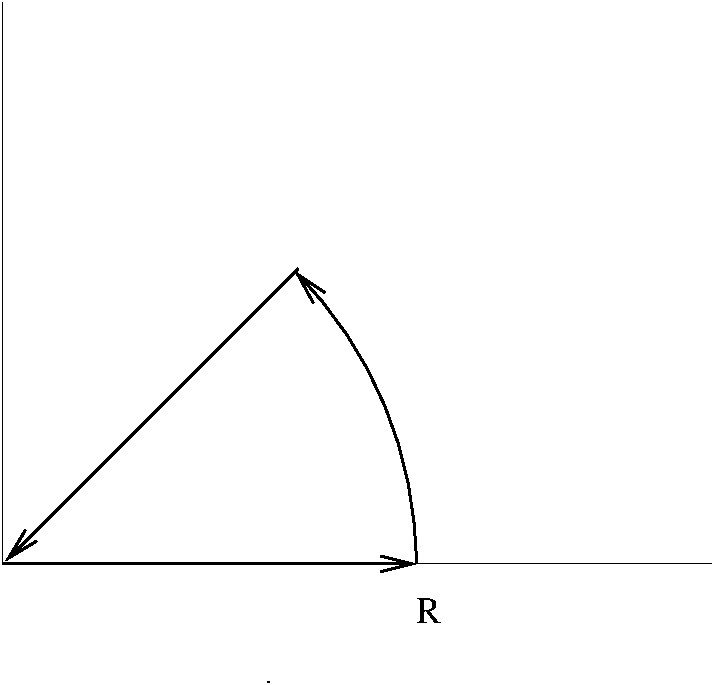
\includegraphics[scale=0.3]{contour_fresnel.pdf}
\caption{Contour $\gamma_r$}\label{fig:contour2}
\end{figure}
\begin{enumerate}
\item L'application $f$ est holomorphe comme composée d'applications
holomorphes. Sa dérivée est $f^\prime(z) = 2 i z f(z)$, qui est continue. 
\item
Par la formule de Cauchy, on a~:
\[
\int_{\gamma_3 . \gamma_2 . \gamma_1} f(z) dz = 0
\]
Par ailleurs~:
\[
\int_{[0,R]} e^{ix^2}d \lambda(x) = \int_{\gamma_1} f(z) dz
\]
En choisissant pour $\gamma_2$ le paramètrage~:
\[
t \in [0, \frac{\pi}{4}] \to \gamma_2(t) = e^{it}
\]
on obtient~:
\[
\int_{\gamma_2} f(z) dz = \int_{[0, \frac{\pi}{4}]} e^{-R^2 \sin (2t)
+ i R^2 \cos(2t)} i R e^{it} d \lambda(t)
\]
On peut majorer le module de $\int_{\gamma_2} f(z) dz$ par~:
\[
\int_{[0, \frac{\pi}{4}]} e^{-R^2 \sin (2t)}  R d \lambda(t)
\]
Comme l'application $\sin$ est concave sur $[0, \frac{\pi}{2}]$, sur
cet intervalle on a~: $\sin(t) \geq \frac{2 t}{\pi}$, ce qui donne la
majoration~:
\[
\left | \int_{\gamma_2} f(z) dz \right | \leq 
\int_{[0, \frac{\pi}{4}]} e^{-\frac{R^2 4 t}{\pi}} R dt =
\frac{(\pi)(1- e^{-R^2})}{4 R}
\]
\item
\[
\int_{\gamma_3} f(z) dz = e^{i \frac{\pi}{4}} \int_{[0,R]} e^{-t^2} d\lambda(t)
\]
d'où en passant à la limite et en remarquant que $\lim_{R \to
+\infty}\int_{\gamma_2} f(z) dz = 0$~:
\[
I = J = \frac{1}{2} \sqrt{\frac{\pi}{2}}
\]
\end{enumerate}
\begin{fex}
 Soit $f \colon z \in \mathbb{C} \mapsto \exp(-z^2)$.
\begin{enumerate}
  \item Montrer que $f$ est holomorphe dans $\mathbb{C}$, de dérivée continue.
  \item En utilisant le contour $\gamma_r$ donné figure \ref{fig:contour3},
déterminer, pour
  $\omega \in \mathbb{R}$ fixé, la valeur de l'intégrale:
  \[
  \int_{\gamma_r} \exp(-z^2)dz
  \]
  \item En faisant tendre $r$ vers $+\infty$ et en faisant un raisonnement
  similaire à celui de l'exercice précédent, déterminer la transformée de
  Fourier de l'application $x \mapsto \exp(-x^2)$.
\end{enumerate}
\end{fex}
 \begin{figure}[ht]
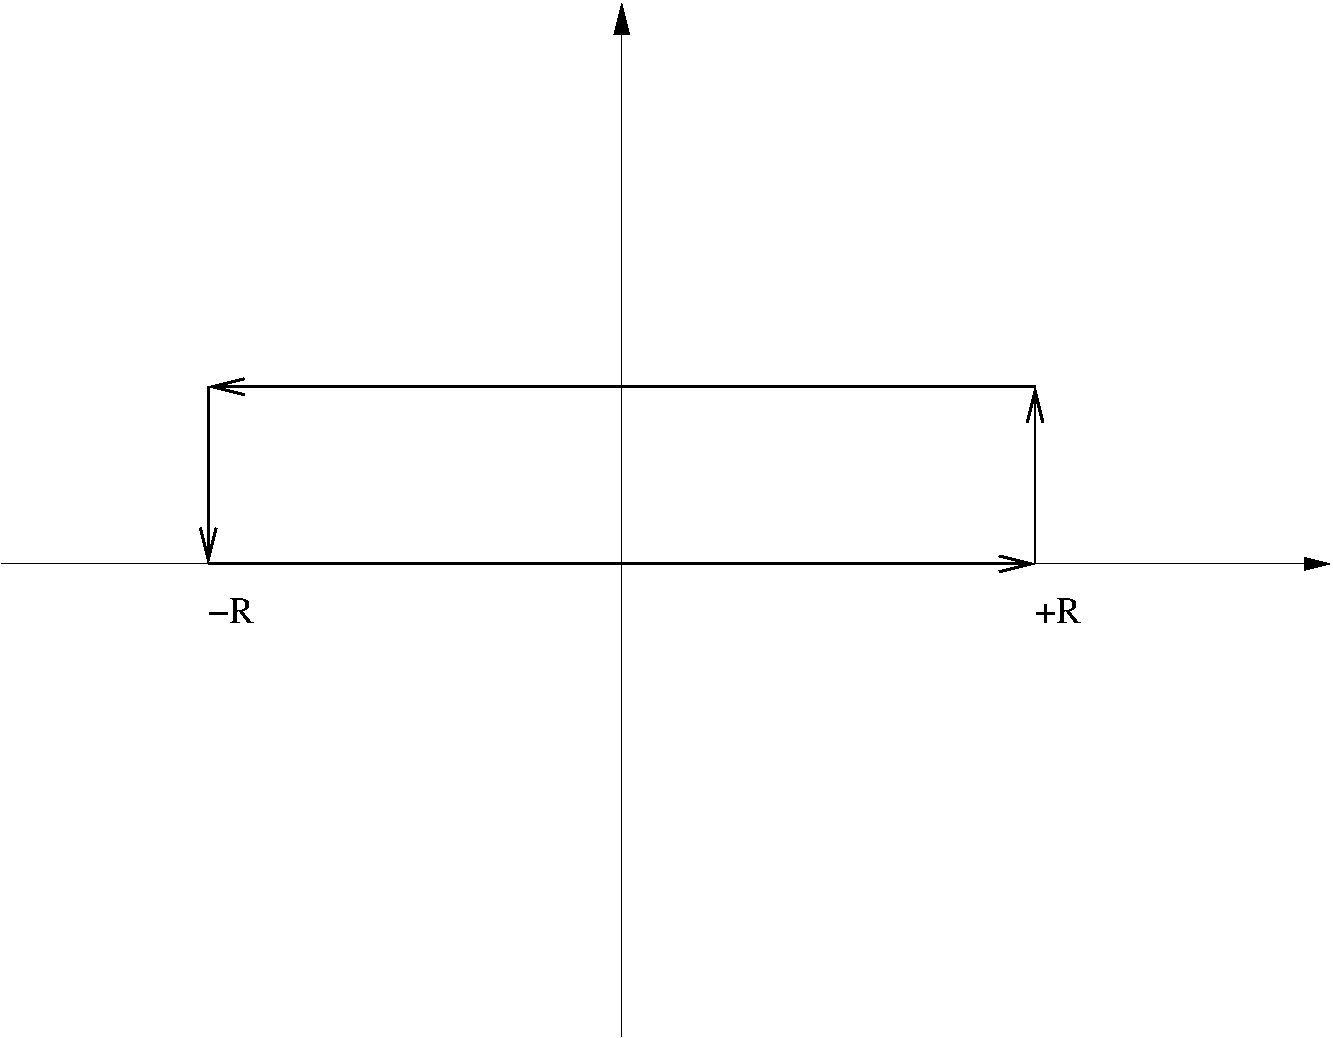
\includegraphics[scale=0.3]{contour_gauss.pdf}
\caption{Contour $\gamma_r$}\label{fig:contour3}
\end{figure}
\begin{enumerate}
 \item Même raisonnement que dans l'exercice précédent.
\item L'application intégrée est holomorphe, la formule de Cauchy s'applique:
\[
  \int_{\gamma_r} \exp(-z^2)dz = 0
  \]
\item L'intégrale sur l'axe réel est:
\[
 \int_{[-r,r]} \exp(-x^2) dx 
\]
de limite $\sqrt{\pi}$ pour $r \to +\infty$. Le segment supérieur se paramètre
par:
\[
 t \in [-r,r] \mapsto -t+i \frac{\omega}{2}
\]
L'intégrale le long de ce chemin est donc:
\[
 - \int_{[-r,r]} e^{-t^2 + i t \omega + \frac{\omega^2}{4}} dt
\]
La limite lorsque $r\to +\infty$ est:
\[
- e^{\frac{\omega^2}{4}} \int_\R  e^{-t^2 + i t \omega} dt 
\]

Finalement, l'intégrale sur les segments verticaux aura pour limite $0$ si $r
\to +\infty$. Un paramétrage possible du segment situé en $r$ est:
\[
t \in [0, \frac{\omega}{2}] \mapsto r + it 
\]
conduisant à l'intégrale:
\[
 i \int_{[0, \frac{\omega}{2}]} e^{-(r+it)^2} dt 
\]
son module se majore par:
\[
 \frac{\omega}{2}e^{-r^2 + \frac{\omega^2}{4}}
\]
qui a bien pour limite $0$ lorsque $r \to +\infty$. Le second segment vertical
se traite de la même façon. En regroupant les termes et en remarquant que la
transformée de Fourier est une application paire, on en déduit finalement
qu'il s'agit de l'application:
\[
 \xi \mapsto \sqrt{\pi} e^{-\frac{\omega^2}{4}}
\]
\end{enumerate}
\begin{fex}
Soit $f$ l'application définie par:
\[
f \colon z \mapsto \frac{\exp(iaz)}{1+z^2}
\]
avec $a>0$ réel. 
\begin{enumerate}
  \item En utilisant la première formule de Cauchy, évaluer l'intégrale de $f$
  le long du contour donné figure \ref{fig:contour_ex1} et sous l'hypothèse
  $R>1$.
  \item Par passage à la limite $R \to +\infty$, en déduire la transformée de
  Fourier de l'application $x \mapsto (1+x^2)^{-1}$.
\end{enumerate}
\end{fex}
\begin{figure}[ht]
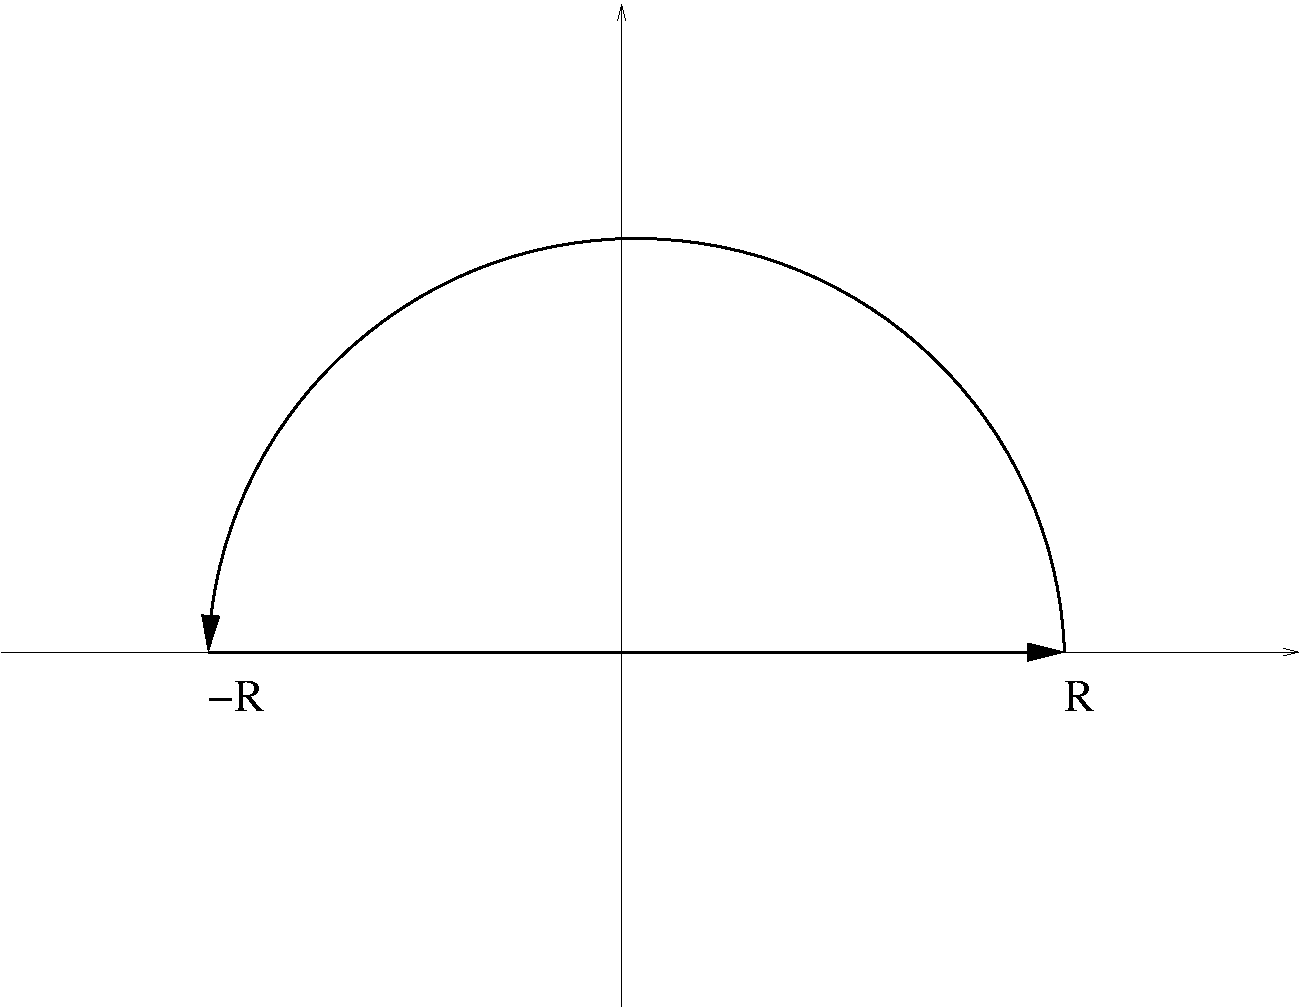
\includegraphics[scale=0.3]{contour_ex1.pdf}
\caption{Contour d'intégration}\label{fig:contour_ex1}
\end{figure}
\begin{enumerate}
 \item Pour $R > 1$, le point $i$ se trouve à l'intérieur du contour
d'intégration $\gamma$. On a donc:
\[
 \int_\gamma \frac{\exp(iaz)}{z+i} \frac{dz}{z-i} = i 2 \pi \frac{\exp(-a)}{2i}
= \pi \exp(-a)
\]
\item On applique le lemme de Jordan:
\[
\left|z\frac{\exp(iaz)}{z^2+1}\right| = \frac{|z|\exp(-a\Im(z))}{|1+z^2|}
\]
Sur le demi-cercle, $\Im(z) \leq 0$, d'où:
\[
\frac{|z|\exp(-a\Im(z))}{|1+z^2|} \leq \frac{R}{R^2-1}
\]
qui a pour limite 0 lorsque $R \to +\infty$.
\item On obtient immédiatement que pour $\xi > 0$, la transformée de Fourier a
pour valeur $\pi \exp(-\xi)$. Par parité, elle vaut donc sur tout $\R$,
$\pi \exp(-|\xi|)$.

\end{enumerate}
\begin{fex}
 Calculer l'intégrale généralisée~:
\[
I = \int_0^{+\infty} \frac{x^2 \cos(ax)}{1+x^4} dx , \quad a \in
\mathbb{R}
\]
\end{fex}
L'intégrale est absolument convergente~:
\[
\left |  \frac{x^2 \cos(ax)}{1+x^4} \right | \leq \frac{x^2}{1+x^4}
\]
On supposera $a\geq0$ en toute généralité puisque le cosinus est une application
paire.
Soit $f_1 : z \to \frac{z^2 e^{iaz}}{1+z^4}$ que l'on intègre sur le contour
de l'exercice précédent.
Le lemme de Jordan s'applique directement sur le demi-cercle~:
\[
\left |
\frac{z^3 e^{iaz}}{1+z^4} 
\right | \leq \frac{|z|^3 e^{-a \Im(z)}}{|1-|z|^4|}
\]
Les pôles de $f$ dans le domaine intérieur au contour sont, pour $R$ assez
grand~:
\[
z_1 = e^{i\frac{\pi}{4}}, \, z_2 = e^{i\frac{3\pi}{4}}
\]
On utilise la formule du cours pour calculer le résidu d'une fraction
rationnelle en un pôle simple~: 
\[
Res(z_k) = \frac{z_k^2 e^{ia z_k}}{4 z_k^3}
\]
On en déduit après calculs~:
\[
I = \frac{\pi e^{-a/\sqrt{2}}}{2\sqrt{2}} \left (
\cos\frac{a}{\sqrt{2}} - \sin \frac{a}{\sqrt{2}} \right )
\]

\begin{fex}
 Calculer l'intégrale généralisée~:
\[
I = \int_0^{+\infty} \frac{ \sin x}{x}dx
\]
\end{fex}
On utilise l'application $g : z \to \frac{e^{iz}}{z}$ et le contour $\gamma$ donné en
figure \ref{fig:contour_sinc}. 
$g$ est
holomorphe dans le domaine intérieur au contour on a donc:
\[
\int_{\gamma} g(z) dz = 0
\]

Par continuité
de $g$, la  limite de l'intégrale
Le demi-cercle de rayon intérieur de rayon $\epsilon$, noté $\gamma_4$, se paramètre par:
\[
t \in [0,\pi] \mapsto \epsilon e^{it}
\]
On peut évaluer l'intégrale de $g$ le long de $\gamma_4$ avec la formule vue en cours:
\[
\int_{\gamma_4}^{} g(z) dz = \int_0^\pi \frac{e^{i\epsilon(\cos t + i \sin t)}}{\epsilon e^{it}}i \epsilon e^{it}dt = i \int_0^\pi e^{i\epsilon(\cos t + i \sin t)} dt
\]
Le théorème de convergence dominée s'applique, on en déduit que la limite de cette intégrale pour $\epsilon$ tendant vers 0 est $i \pi$. Dans le contour $\gamma$, le demi-cercle est parcouru en sens inverse, on devra donc prendre $-i \pi$. 
Sur le
demi-cercle extérieur (de rayon $R$), on majore l'intégrale (voir exercice 2.6) par~:
\[
2 \int_{[0, \frac{\pi}{2}]} e^{- \frac{2 R t}{\pi}} d\lambda(t)
\]
prouvant que la limite est $0$ lorsque $R$ tend vers l'infini\footnote{on peut également utiliser la convergence dominée après un 
paramétrage du demi-cercle}.
 On obtient finalement que la valeur de
l'intégrale généralisée demandée est $\frac{\pi}{2}$.
\begin{figure}[ht]
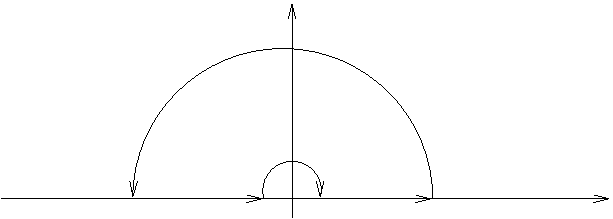
\includegraphics[scale=1]{contour_sinc.pdf}
\caption{Contour d'intégration}\label{fig:contour_sinc}
\end{figure}
\end{document}